\chapter[Introduction]{Introduction}
\section{Motivation}
Humankind has only a few ways to generate reliable, nonintermittent 
base load power: fossil fuels, hydro-power, geothermal power, and 
nuclear energy. Because of increasing global warming and climate 
change concerns, sources with negligible CO$_2$ footprints 
are crucial measures for global temperature change control. 
From an environmental viewpoint, hydro and nuclear power are 
preferable ways to generate reliable power. Nevertheless, the 
potential for a hydro-power is strictly limited by local geographical 
conditions, hence, the only option left is nuclear power. Nuclear 
power plants generate 4.9\% of global energy \cite{noauthor_key_2017}. 
Moreover, a nuclear share in energy generation is projected to stay 
constant through 2040 while electricity demand will 
increase by 30\% \cite{noauthor_world_2017}. Unfortunately, a negative 
public attitude to nuclear was formed in many developed countries 
because of concerns regarding safety, nuclear weapons 
proliferation, radioactive waste treatment, and competitiveness with 
other sources of energy (i.e. renewables). This negative public 
attitude to nuclear energy makes it challenging to justify its zero 
emissions benefits.

Generation IV International Forum (GIF) chose \glspl{MSR} among the 
six advanced reactor concepts for further research and development. 
\glspl{MSR} 
offer significant improvements ``in the four broad areas of 
sustainability, economics, safety and reliability, and proliferation 
resistance and physical protection" \cite{doe_technology_2002}. To 
achieve the goals formulated by the GIF, \glspl{MSR} 
simplify the reactor core and improve inherent safety by using 
liquid coolant which is also a fuel\footnote{Herein \glspl{MSR} are 
assumed to be reactors with liquid fuel which simultaneously serves 
as coolant.}. In a thermal spectrum \gls{MSR}, liquid fuel is consists 
of carrier salt (i.e. LiF or LiF-BeF$_2$) and fluorides of fissile 
and/or fertile materials (i.e. UF$_4$, PuF$_3$ and/or ThF$_4$) 
which is circulates in a loop-type primary circuit 
\cite{haubenreich_experience_1970}. 
This innovation leads to immediate advantages over traditional, 
solid-fueled, reactors. These include near-atmospheric pressure 
in the primary loop, relatively high coolant temperature, outstanding 
neutron economy, a high level of inherent safety, reduced fuel 
preprocessing, the ability to continuously remove fission products 
and add fissile and/or fertile elements without shutdown 
\cite{leblanc_molten_2010}. The possibility of continuously removing 
neutron poisons increases the potential fuel burnup and thus 
improves the resource utilization of \glspl{MSR}. Finally, the \gls{MSR} 
also could be employed for transmutation of 
spent fuel from current \glspl{LWR} \cite{fratoni_design_2004}.

Recently, interest in \glspl{MSR} has resurged, with multiple new companies 
pursuing commercialization of \gls{MSR} designs\footnote{Examples 
include liquid-fueled molten salt designs from Terrapower, Terrestrial, 
ThorCon, Flibe, Copenhagen Atomics, Elysium, etc.}. China's \gls{MSR} program 
was initiated in 2011 and promises to startup a 2MW$_{th}$ 
liquid-fueled test \gls{MSR} in 2020, a 10MW$_{th}$ 
demonstration reactor in 2025, and a gigawatt-level 
commercial reactor in 2050 \cite{zhang_review_2018}. The European 
Union funds the Safety Assessment of the Molten Salt Fast Reactor 
(SAMOFAR) project, in which several European research institutes and 
universities are developing various molten salt reactor prototypes 
such as the \gls{MSFR} \cite{fiorina_molten_2013} and the \gls{MOSART} 
\cite{ignatiev_molten_2014}.
To advance these \gls{MSR} concepts, particularly with respect 
to their strategies for online reprocessing and refueling, 
computational analysis methods capturing their unique reactor physics 
and process chemistry are needed. To correctly determine properties and 
operation conditions of \glspl{MSR}, including injection/removal schemes, 
computational tools to accurately model the processes which are unique for 
this particular reactor type. 

The main objective of the proposed work is to develop the online 
reprocessing simulation package, SaltProc, which couples with the 
continuous-energy Monte Carlo depletion calculation code, Serpent 2 
\cite{leppanen_serpent_2015}, for liquid-fueled \gls{MSR} depletion 
simulations. The ultimate objective of this effort is to develop a generic 
open-source tool capable of simulating a wide range of liquid-fueled 
systems, including two-fluid, multi-region designs, and validate it against 
existing modeling efforts. 

This document outlines the motivation, preliminary work, and future work 
proposed towards developing a simulation tool for analyzing fuel depletion in 
a liquid-fueled \glspl{MSR}. Chapter 1 serves as a literature review, 
providing background on fuel burnup, online fuel reprocessing approaches, 
safety parameters evolution during the reactor operation, and how these 
concepts have been applied to a wide range of \glspl{MSR} in the literature. 
Chapter 2 covers modeling online reprocessing details, including proposed 
software architecture, \gls{VV} method, demonstration cases, safety 
parameters evolution, and preliminary results. Specifically, these 
demonstration and verification efforts will 
focus on the \gls{TAP} \gls{MSR} because it well analyzed in the literature. 
Finally, Chapter 3 summarizes the conclusions reached concerning the 
appropriate mechanical and chemical models of fuel processing 
components to utilize in the online reprocessing plant simulation. 
Additionally, Chapter 3 outlines simulations plan for analyzing operational 
and safety characteristics evolution during \gls{TAP} reactor lifetime. 
Finally, remaining future work and expected contributions to the 
nuclear community will be summarized.

\section{Fuel burnup and online reprocessing}
All liquid-fueled \gls{MSR} designs involve varying levels of online fuel 
processing. Minimally, volatile gaseous fission products (e.g., Kr, Xe) 
escape from the fuel salt during routine reactor operation and must be 
captured. Additional systems might be used to enhance the removal of those 
elements. Most designs also call for the removal of rare earth metals from 
the core since these metals act as neutron poisons. Some designs suggest a 
more elaborate list of elements to process (figure~\ref{fig:periodic_tab}), 
including the temporary removal of protactinium from the salt or other 
regulation of the actinide inventory in the fuel salt 
\cite{ahmad_neutronics_2015}. Fresh fuel salt with dissolved fissile and/or 
fertile material (e.g., $^{233}$U, $^{232}$Th, \gls{LEU}, a transuranic 
vector from \gls{LWR} \gls{SNF}) make-up the salt mass loss caused by poisons 
removal and conserves the total mass in the primary loop.
\begin{figure}[htp!] % replace 't' with 'b' to 
  \centering
  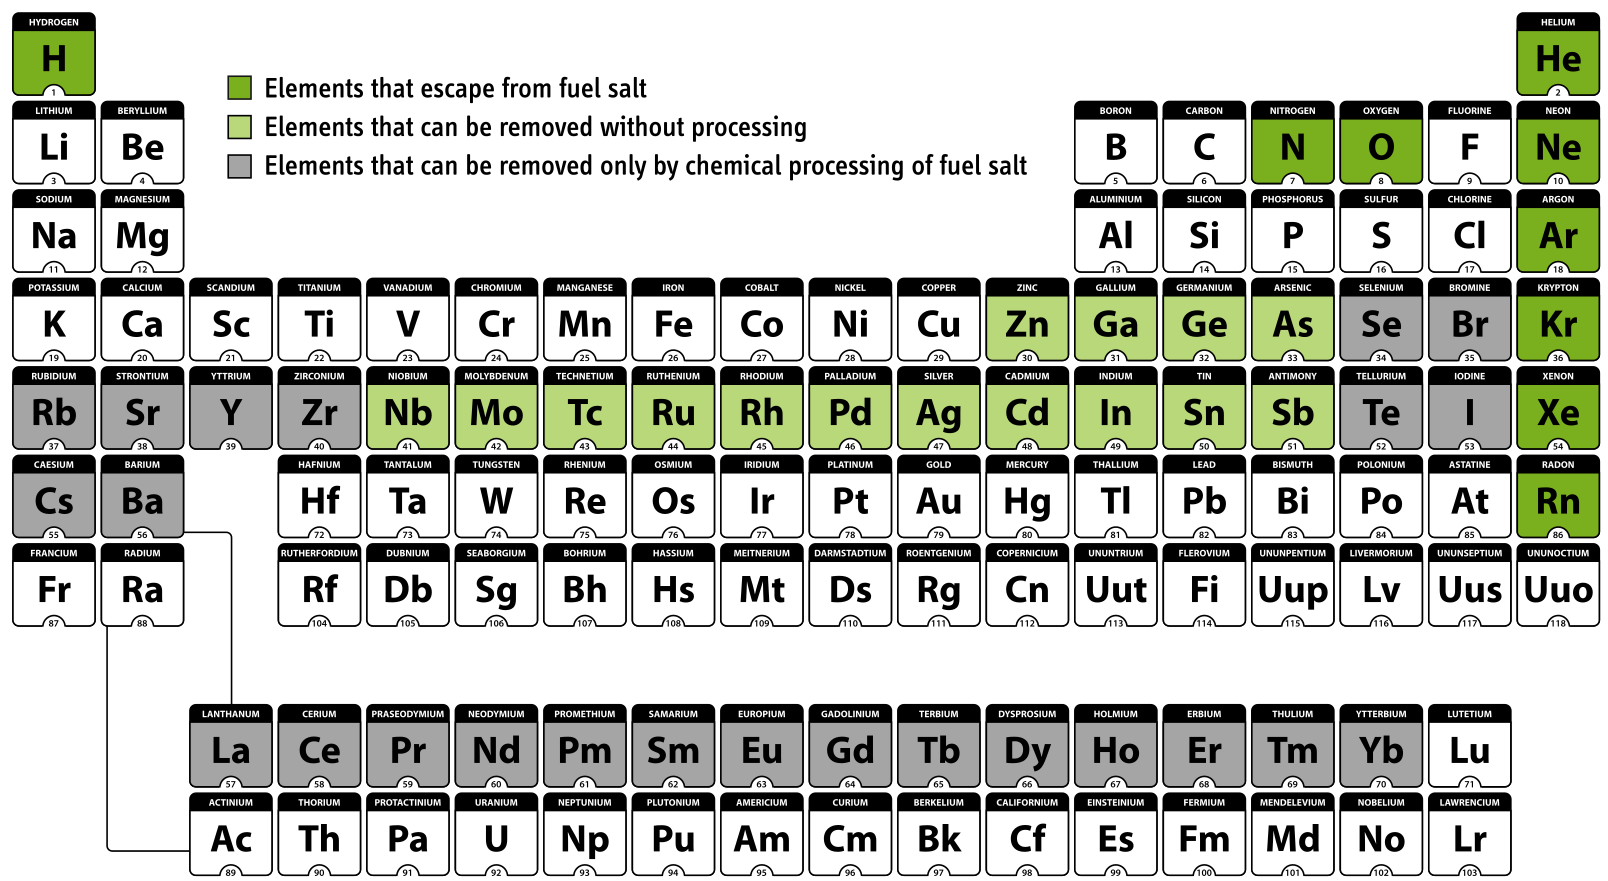
\includegraphics[width=0.9\textwidth]{periodic_map.png}
  \caption{Processing options for \gls{MSR} fuels (figure reproduced from 
  Ahmed \emph{et al.} \cite{ahmad_neutronics_2015}).}
  \label{fig:periodic_tab}
\end{figure}

Most of the liquid-fueled nuclear reactors adopted nonintermittent 
separations and feeds: the core material is moved to or from the core at all 
times (continuous) or specific intervals (batch). Contrarily, in a 
solid-fueled reactor, fission products and actinides 
remain within the initial fuel material during and after operation until 
reprocessing. The ability to perform online fuel salt reprocessing improves 
the potential neutronic performance of liquid-fueled reactors. First, it 
is unnecessary for liquid-fueled reactors to operate with excess reactivity 
because fissile material is continuously being added to the core. Second, 
continuously removing fission products, including strong absorbers (poisons) 
should significantly improve fuel utilization and decrease parasitic 
neutron absorption. Finally, for a breeder (reactor with a 
\gls{CR}\footnote{\gls{CR} $\equiv$ fissile generated/fissile consumed: if CR 
$<$ 1, the reactor is a ``converter''; CR $\equiv$ 1, an ``isobreeder''; 
CR $>$ 1, a ``breeder.''}$>1$, excess of fissile material might be 
continuously evacuated from the core and used to startup new reactors. 
Nevertheless, the removal of each element from the liquid fuel salt presents 
a unique challenge in terms of chemical separation, storage, and disposal of 
the separated materials.

Continuous fuel salt reprocessing prevents the usage of most contemporary 
nuclear reactor fuel burnup software. Few code packages were developed 
specifically for \gls{MSR} depletion simulations at universities and research 
institutions and not available for external use. The foundation for these 
in-house tools was based on early \gls{MSR} simulation methods at \gls{ORNL}, 
which integrated neutronic and fuel cycle codes (i.e., Reactor Optimum Design 
(ROD) \cite{bauman_rod_1971}) into operational plant tools (i.e., Multiregion 
Processing Plant (MRPP) \cite{kee_mrpp_1976}) for \gls{MSR} and reprocessing 
system design. A summary of recent efforts is listed in 
table~\ref{tab:msr_codes}.
\begin{table}[t]
\fontsize{9}{11}\selectfont
\caption{Tools and methods for liquid-fueled \glspl{MSR} fuel salt depletion 
analysis.}
\begin{tabularx}{\textwidth}{X X X X X} 
\hline 
&Nuttin \emph{et al.}, 2005 \cite{nuttin_potential_2005}& Aufiero \emph{et al.}, 
2013 \cite{aufiero_extended_2013} & Betzler \emph{et al.}, 2018 
\cite{betzler_fuel_2018}&Proposed work \\ [12pt]
\hline
Neutron transport software & \gls{MCNP} & Serpent 2 & SCALE6.2 & Serpent 2 \\ 
[12pt]
Neutron transport method & \multicolumn{2}{c}{Monte Carlo continuous energy} & 
Deterministic discrete ordinates & Monte Carlo continuous energy \\ [12pt]
Burnup software & REM (in-house) code & Serpent 2 & ORIGEN-S & Serpent 2 \\ 
[12pt]
Geometry model & three cells & full-core 3D & unit cell & full-core 3D\\ [12pt]
\gls{FP} removal/feed  & continuous &continuous & batch-wise & batch-wise\\ 
[12pt]
Separation efficiency &\multicolumn{3}{c}{constant, must be determine by user 
before simulation} & dynamic \\ [12pt]
Fuel reprocessing plant & \multicolumn{3}{c}{single component, ``black'' box 
model} & realistic multi-component model\\ [12pt]
Reactivity control & \multicolumn{2}{c}{continuous adjustment of fissile 
material injection} & batch injection of fissile material & periodical 
adjustment of geometry and fissile material injection\\
\hline
\end{tabularx}
  \label{tab:msr_codes}
\end{table}

Two main online reprocessing simulation approaches are commonly used in the 
literature: materials move to and from the core continuously or at specific 
time steps (batch-wise). In the batch-wise approach, the burnup simulation 
stops at a given time and restarts with a new liquid fuel composition 
(after removal of discarded materials and addition of fissile/fertile 
materials).

Recently, Nuttin \emph{et al.} developed in-house 
depletion code REM which directly couples with the \gls{MCNP}  
\cite{noauthor_mcnp_2004} to simulate fuel salt material evolution in 
simplified \gls{MSBR}-like reactor. That work directly integrated
Bateman differential equations using neutron flux from the \gls{MCNP}, 
tracking all the isotopes available in the data library, and control 
reactivity to maintain reactor critical \cite{nuttin_potential_2005}.

In a similar vein, Aufiero \emph{et al.} extended Serpent 2 for continuous 
reprocessing simulations by explicitly introducing ``reprocessing'' time 
constants into the system of Bateman equations and adding effective decay and 
transmutation terms for each nuclide \cite{aufiero_extended_2013}. The 
developed extension directly accounts for the effects of online fuel 
reprocessing on depletion calculations and features a reactivity control 
algorithm. The extended version of SERPENT2 was assessed against a dedicated 
version of the deterministic ERANOS-based EQL3D procedure in 
\cite{fiorina_investigation_2013} and applied to analyze the \gls{MSFR} fuel 
salt isotopic evolution.

%I employed this built-in Serpent 2 sub-routine for a simplified unit-cell 
%geometry of the thermal spectrum thorium-fueled \gls{MSBR} and found it 
%impossible to use \cite{rykhlevskii_online_2017}. Primarily, it is 
%undocumented, and the discussion forum for Serpent users is the only useful 
%source of information at the moment. Additionally, the reactivity control 
%module described in Aufiero \emph{et al.} is not available in the latest 
%Serpent 2.1.31 release. Third, mass conservation in the loop is hard to 
%achieve due to different unit for removal and feed. 

\gls{ORNL} researchers have developed ChemTriton, a Python script for
SCALE/TRITON which uses the batch-wise approach to simulate a continuous 
reprocessing and refill for either single or multiple fluid designs. 
ChemTriton models salt treatment, separations, discharge, and refill using a 
unit-cell MSR SCALE/TRITON depletion simulation over small time steps to 
simulate continuous reprocessing and deplete the fuel salt 
\cite{powers_new_2013, betzler_fuel_2018}.

Most of existing tools represented fuel salt reprocessing plant as a static 
``black box'' model which removes target elements all at once with static 
efficiency, determined by user before start the depletion simulation. 
Typical inputs and outputs for this ``black box'' model are vectors of 
elements and extraction efficiencies and can be expressed as follows:
\begin{equation}
\begin{bmatrix}
N^{in}_{0} \\ \vdots \\ N^{in}_{e} \\ \vdots \\ N^{in}_{E} \\
\end{bmatrix} 
\times
\begin{bmatrix}
\epsilon_{0} \\ \vdots \\ \epsilon_{e} \\ \vdots \\ \epsilon_{E} \\
\end{bmatrix} =
\begin{bmatrix}
N^{out}_{0}\\ \vdots \\ N^{out}_{e} \\ \vdots \\N^{out}_{E}  \\
\end{bmatrix}
\end{equation}
where $N^{in/out}$ is the number density of atoms and $\epsilon$ is the 
extraction efficiency for all elements $e$ in $(0, E)$. Main issues related 
with static ``black box'' model assumptions in the literature: 
\begin{enumerate}
	\item The separation efficiency vector must be immutable with time but  
	long-term depletion simulation might require a time-dependent extraction 
	efficiency vector.
	\item The separation efficiency independent of the reactor operational 
	parameters but the efficiency might changes with temperature, power level, 
	current fuel salt isotope composition, and material mass flow rate.
	\item All reprocessing plant components are treated as a single component 
	but the fuel salt in a reprocessing plant undergoes many separate components 
	(e.g. helium bubbling, nickel mesh filter, etc) which target specific 
	elements. Some of these components can be connected in series, parallel, or 
	series-parallel. The ``black box'' model (only single process) requires 
	massive pre-simulation analytic work from the user to calculate lumped 
	separation 	efficiency vector before a simulation is run and cannot be 
	adjusted during simulation.	
\end{enumerate}

Some of tools listed in table~\ref{tab:msr_codes} used major approximations 
that may lead to inaccurate fuel evolution predictions, others are not 
available for external users. Therefore, a purpose-made, open-source 
simulation package, SaltProc, which expands the capability of the 
continuous-energy Monte Carlo 
Burnup calculation code, Serpent 2, for simulation liquid-fueled \gls{MSR} 
operation is proposed in this Chapter.

\subsection{Operational and safety parameters evolution}
In contrast with conventional solid-fueled reactors, which are require a 
complete fuel replacement every 4-5 years\footnote{For the most common 
18-month cycle, 
during refueling personnel removing 1/3 of the fuel assemblies, re-arranging 
other assemblies, and loading fresh fuel into the core. Thus, any fuel 
assembly is kept in the core at most $3\times 18=54$ months.}, the initial 
fuel salt batch stays in the \gls{MSR} reactor primary loop during whole 
lifetime. Therefore, the fuel salt accumulating \glspl{FP}, not captured 
by fuel  reprocessing system, and transuranic elements\footnote{The chemical 
elements with atomic numbers greater than uranium (92).}. 
Continuous variation of fuel salt composition have a significant influence on 
the neutron energy spectrum and, consequently, affects the reactor behavior 
and rises significant safety concerns.

Nuttin {et al.} studied evolution of key safety parameter: temperature  
coefficient, and estimated it at start-up and at equilibrium state. The 
temperature coefficient 
quantify reactivity changes due to accidental temperature increase in the 
core and was calculated in that work as:
\begin{align}
& \qquad\qquad \alpha = \frac{k_{1200} - k_{900}}{\delta T} 
\intertext{where}
k_{900}, k_{1200}  &= \mbox{the multiplication coefficient for 900K and 1200K} 
\nonumber \\
\delta T &= 1200K-900K \nonumber
\end{align}
That work showed negative and decreasing during reactor operation fuel 
temperature 
coefficient ($-1.5$ and $-1.0pcm/K$ at start-up and at equilibrium state, 
respectively); they also reported positive and invariable with respect to time 
total 
temperature coefficient ($\approx+0.8pcm/K$) \cite{nuttin_potential_2005}. 
Recently, Park and colleagues expanded Nuttin' approach to a full-core 
high-fidelity \gls{MSBR} model and estimated safety parameters evolution over 20 
years of operation. These calculations showed relatively large negative total 
temperature coefficient during 20 years of the reactor operation; the 
coefficient magnitude weaken from $-3.21$ to $-1.41pcm/K$ at start-up and at 
equilibrium composition, respectively. Additionally, that work reported control 
rod effectiveness deterioration due to neutron spectrum hardening during reactor 
operation \cite{park_whole_2015}. 

More recently, Betzler \emph{et al.} reported key safety parameters evolution 
for \gls{TAP} \gls{MSR}: the fuel reactivity coefficient at \gls{BOL} and 15 
years from \gls{BOL} are negative and decreasing slowly  over the reactor 
lifetime; the moderator reactivity coefficient is small and positive at 
\gls{BOL}, and became negative after 15 years of operation. Overall, thermal 
feedback seems to be stronger in the \gls{TAP} reactor and deteriorates 
insignificantly during the reactor operation. Notably, authors ignored materials 
densities change with temperature to simplify temperature coefficients 
calculation (e.g., only  Doppler broadening has been taken into account). The 
researchers also calculated total worth of all control rods in the \gls{TAP} 
core at start-up only \cite{betzler_assessment_2017}. 

The evolution of control rod worth in the \gls{TAP} was never reported in the 
literature before. The proposed work will illuminate evolution of major safety 
parameters (fuel, moderator and total temperature coefficient, void reactivity 
coefficient, control rod worth) for the \gls{TAP} \gls{MSR} at various moments 
during the reactor operation.
%during 60 years of reactor lifetime. Additionally, impact of neutron poisons 
accumulation in the fuel salt during short-term transients (i.e. load-following) 
on safety characteristics will be investigated.

\subsection{Chapter Conclusion}
The State-of-the-Art software packages and methods for depletion analysis of 
liquid-fueled \gls{MSR} and evolution of safety parameters are reviewed in this 
Chapter. Based on this summary, I have identified few possible directions for 
the \gls{MSR} tools improvement:
\paragraph{Reproducibility/code availability.} Only Serpent built-in online 
reprocessing feature is included in distribution package and widely available 
for use; other mentioned tools are developed inside research institutions or 
universities and unaccessible for external users. In the era of GitHub 
\cite{github_github_2015} and international scientific collaboration, open and 
reproducible software practices must be implemented to resolve nuclear 
engineering simulation challenges presented by new reactor designs.
\paragraph{Realistic fuel reprocessing system model instead of ``black box''.} 
Major approximations in fuel reprocessing parameters deteriorates fuel salt 
composition predictions; evolution of safety parameters accuracy is toughly 
related to fuel salt composition. Realistic fuel reprocessing system model will 
allow to optimize reprocessing component parameters, collect detailed data about 
waste streams, advance the reprocessing system design.
\paragraph{Constant extraction efficiency.}
\paragraph{Reactivity control.} Reconfigurable moderator configuration in the 
\gls{TAP} core presents a challenge because the core geometry changes with 
respect to time. The reactivity control module which adjusts the core geometry 
to maintain criticality would be a great capability for simulating a new, more 
advanced \gls{MSR} concepts and a short-term transients.
\paragraph{Safety characteristics evolution during reactor operation.} The 
\glspl{MSR} fuel salt  accumulates \gls{FP} and transuranic elements which 
significantly shift neutron energy spectrum. Neutron energy hardening might 
worsen the core safety during operation. The impact of the fuel salt evolution 
on the \gls{MSR} safety parameters must be carefully investigated and reported.

The proposed work will hopefully overcome these issues and demonstrate the tool 
capabilities for promising \gls{TAP} \gls{MSR} concept.